\documentclass[11pt,a4paper]{article}
\usepackage{iftex}
\ifPDFTeX
  \usepackage[utf8]{inputenc}
  \usepackage[T1]{fontenc}
  \usepackage{lmodern}
\else
  \usepackage{fontspec}
  \setmainfont{lmroman10-regular.otf}[BoldFont=lmroman10-bold.otf,ItalicFont=lmroman10-italic.otf,BoldItalicFont=lmroman10-bolditalic.otf]
\fi
\usepackage[slovene]{babel}
\usepackage{graphicx,geometry,hyperref}
\geometry{margin=24mm}
\hypersetup{colorlinks=false,hypertexnames=false,pdfborder={0 0 0},pdftitle={ByteFix: pregled obstoječih rešitev},pdfauthor={Žiga Trbovšek, Leo Dragić, Anže Pečak}}
\setlength{\parindent}{0pt}
\setlength{\parskip}{7pt}
\renewcommand{\figurename}{Slika}
\begin{document}
\begin{titlepage}
\centering
\vspace*{24mm}
{\large KIDS -- skupinski projekt\par}
\vspace{14mm}
{\Huge\bfseries ByteFix\par}
\vspace{7mm}
{\LARGE Pregled obstoječih rešitev\par}
\vspace{9mm}
{\large Predstavitvena spletna stran računalniškega servisa\par}
\vfill
{\large Žiga Trbovšek\\Leo Dragić\\Anže Pečak\par}
\vspace{14mm}
{19. november 2026\par}
\vspace{12mm}
\end{titlepage}

\section{Uvod}
ByteFix je izmišljeno podjetje iz Maribora, ki posameznikom in manjšim podjetjem nudi diagnostiko, popravila in nadgradnje računalnikov ter osnovno IT podporo. Načrtujemo predstavitveno spletno stran, na kateri obiskovalec hitro ugotovi, ali podjetje rešuje njegovo težavo, poišče informativno ceno in najde način za stik.

Problem, ki ga rešujemo, je razpršenost osnovnih informacij o servisu. Uporabnik z okvarjenim računalnikom potrebuje razumljiv opis storitve, pojasnilo o stroških in jasen naslednji korak. V začetnem obsegu bodo štirje zasloni: Domov, Storitve, Cenik ter O nas in kontakt. Kontaktni obrazec bo prikaz vmesnika; dejansko pošiljanje sporočil in rezervacije niso del začetnega obsega.

\subsection{Način pregleda}
Primerjali smo tri javne spletne rešitve slovenskih ponudnikov: ANNI, Mlacom in BBT. Pregled zajema predstavitev storitev, dostopnost cen in kontaktov ter preglednost poti do pomoči. Podatki izhajajo iz uradnih strani \cite{anni,mlacom,bbt}; posnetki zaslona so bili zajeti 19.~novembra 2026.

Prednosti in slabosti so naša ocena prikazanih spletnih vmesnikov glede na potrebe ByteFixa. Ne predstavljajo preizkusa kakovosti popravil, varnosti ali dejanske odzivnosti ponudnikov. Ocenjujemo pregledane strani, ne vseh storitev podjetij.

\subsection{Merila primerjave}
\begin{itemize}
\item Ali obiskovalec hitro prepozna ponujene storitve?
\item Ali sta cenik in pojasnilo stroškov lahko dosegljiva?
\item Ali sta kontakt in naslednji korak jasno predstavljena?
\item Ali navigacija podpira uporabnika, ki potrebuje servis?
\end{itemize}

\newpage
\section{ANNI -- servis računalnikov in opreme}
\textbf{Opis in ključne funkcionalnosti.}
ANNI ima ločeno servisno spletno mesto. Na domači strani so povezave do popravil računalnikov, avdio/video naprav in omrežnih storitev. Glavna navigacija vključuje cenik, podporo in vpogled v servisna popravila. Obiskovalec najde telefon, naslov, delovni čas, kontakt in povezavo za pomoč na daljavo \cite{anni}.

\textbf{Prednosti.}
Servis je ločen od prodaje, zato je namen strani hitro razumljiv. Pomembni kontaktni podatki so izpostavljeni pred opisom storitev. Navigacija poimenuje uporabnikove cilje, na primer iskanje cene ali podpore.

\textbf{Slabosti.}
Po naši oceni majhno besedilo in več hkratnih informacij o delovnem času ter doplačilu otežijo hitro branje. Posamezne servisne kategorije imajo precej opisnega besedila; obiskovalec mora sam izbrati ustrezno pot.

\textbf{Uporaba pri ByteFixu.}
Prevzeli bomo vidne kontakte in neposredno povezavo do cenika. Storitve bomo strnili v kratke kartice, glavno dejanje pa bo povezava na kontaktni obrazec. Vpogleda v servisne naloge ne bomo uvajali.
\begin{figure}[htbp]
\centering
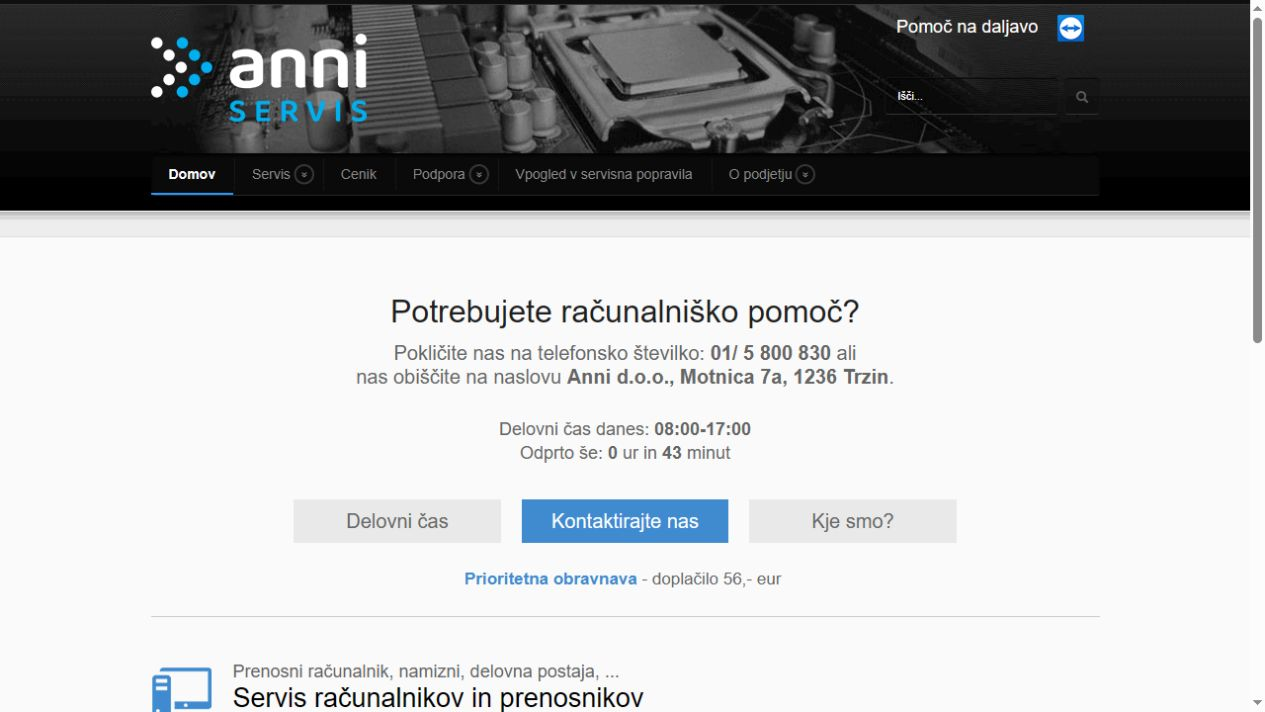
\includegraphics[width=\linewidth,height=83mm,keepaspectratio]{primer_anni.png}
\caption{Domača stran servisa ANNI: kontaktni podatki in navigacija do storitev, cenika in podpore. Lastni posnetek zaslona, 19.~11.~2026 \cite{anni}.}
\label{fig:anni}
\end{figure}

\newpage
\section{Mlacom -- storitve in računalniški servis}
\textbf{Opis in ključne funkcionalnosti.}
Mlacom združuje spletno trgovino in predstavitev servisnih storitev. Na pregledani strani so servisni kontakti, seznam del in cenik, razdeljen po vrstah posegov. Navedene so diagnostika, nadgradnje, programska oprema, omrežja in reševanje podatkov. Stran pojasni tudi upoštevanje stroška diagnostike pri popravilu \cite{mlacom}.

\textbf{Prednosti.}
Obiskovalec dobi konkretne podatke za orientacijo o stroških. Kategorije cenika pomagajo ločiti posege, kontaktni podatki in delovni čas pa so zbrani ob servisni vsebini.

\textbf{Slabosti.}
Naša ocena je, da trgovinske kategorije in ponudba izdelkov podaljšajo pot do servisnih informacij. Dolg besedilni seznam cen zahteva več pomikanja in ima manj izrazito vizualno razmejitev posameznih storitev.

\textbf{Uporaba pri ByteFixu.}
Prevzeli bomo razvrstitev cen po storitvah in pojasnilo, kaj cena vključuje. ByteFix bo imel samostojen cenik s kratko tabelo ter povezavo na povpraševanje. Cene bodo izmišljene in označene kot informativne; ne bomo jih prepisovali od ponudnika.
\begin{figure}[htbp]
\centering
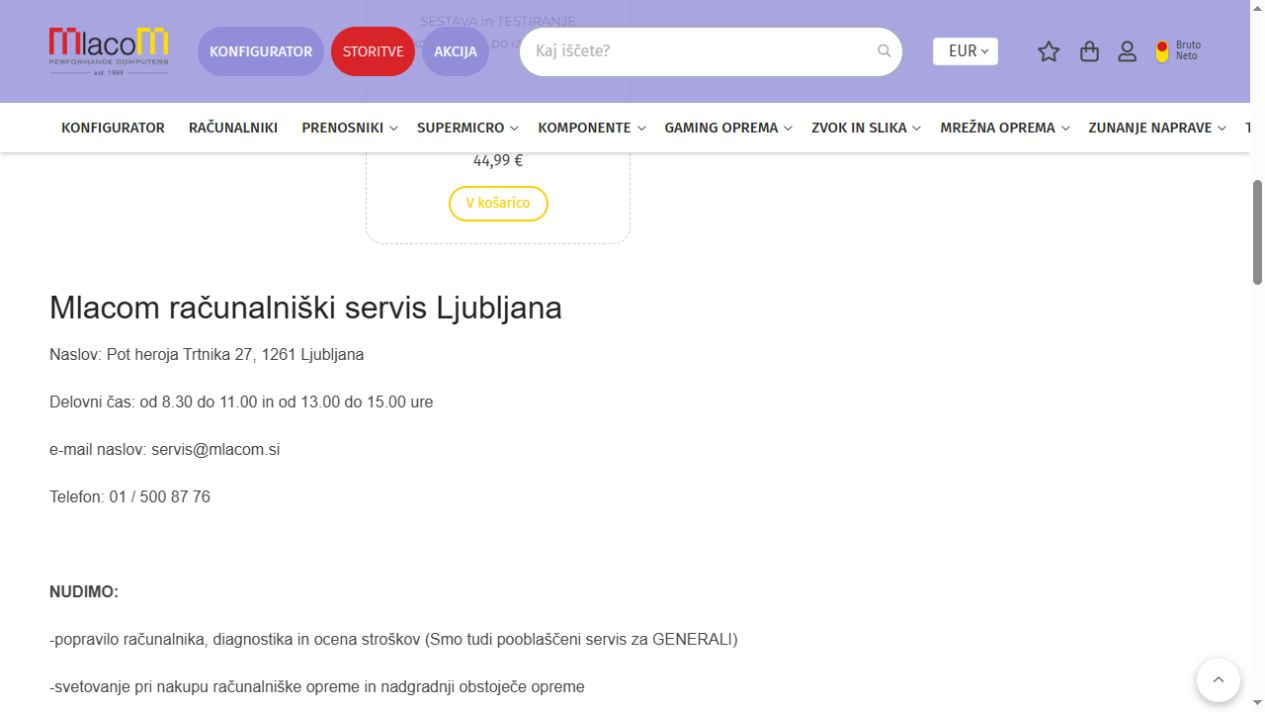
\includegraphics[width=\linewidth,height=83mm,keepaspectratio]{primer_mlacom.png}
\caption{Servisni del strani Mlacom s kontakti in seznamom storitev. Lastni posnetek zaslona, 19.~11.~2026 \cite{mlacom}.}
\label{fig:mlacom}
\end{figure}

\newpage
\section{BBT -- servis računalnikov in računalniške opreme}
\textbf{Opis in ključne funkcionalnosti.}
BBT servis predstavlja znotraj spletne trgovine z obnovljeno računalniško opremo. Stran pojasni postopek ob okvari, kontaktiranje servisa in pomoč na daljavo. Opozori na varnostno kopijo podatkov in izrecno navede, da servisira le opremo, kupljeno pri BBT \cite{bbt}.

\textbf{Prednosti.}
Opis postopka pomaga uporabniku razumeti, kaj naj naredi pred obiskom. Jasno navedena omejitev sprejema opreme zmanjša možnost napačnega pričakovanja. Povezava do cenika dopolnjuje servisne informacije.

\textbf{Slabosti.}
Po naši oceni daljše promocijsko besedilo oteži hitro iskanje praktičnih navodil. Navigacija vsebuje tudi trgovinske vsebine, ki pri iskanju servisa niso nujno pomembne. Omejitev na lastno prodano opremo pomeni, da rešitev ni primerna za vse obiskovalce.

\textbf{Uporaba pri ByteFixu.}
Prevzeli bomo preprost prikaz korakov od kontakta do dogovora o popravilu in opozorilo glede podatkov. ByteFix bo kot izmišljena splošna servisna ponudba namenjen širšemu krogu uporabnikov, pogoje sprejema pa bo jasno opisal.
\begin{figure}[htbp]
\centering
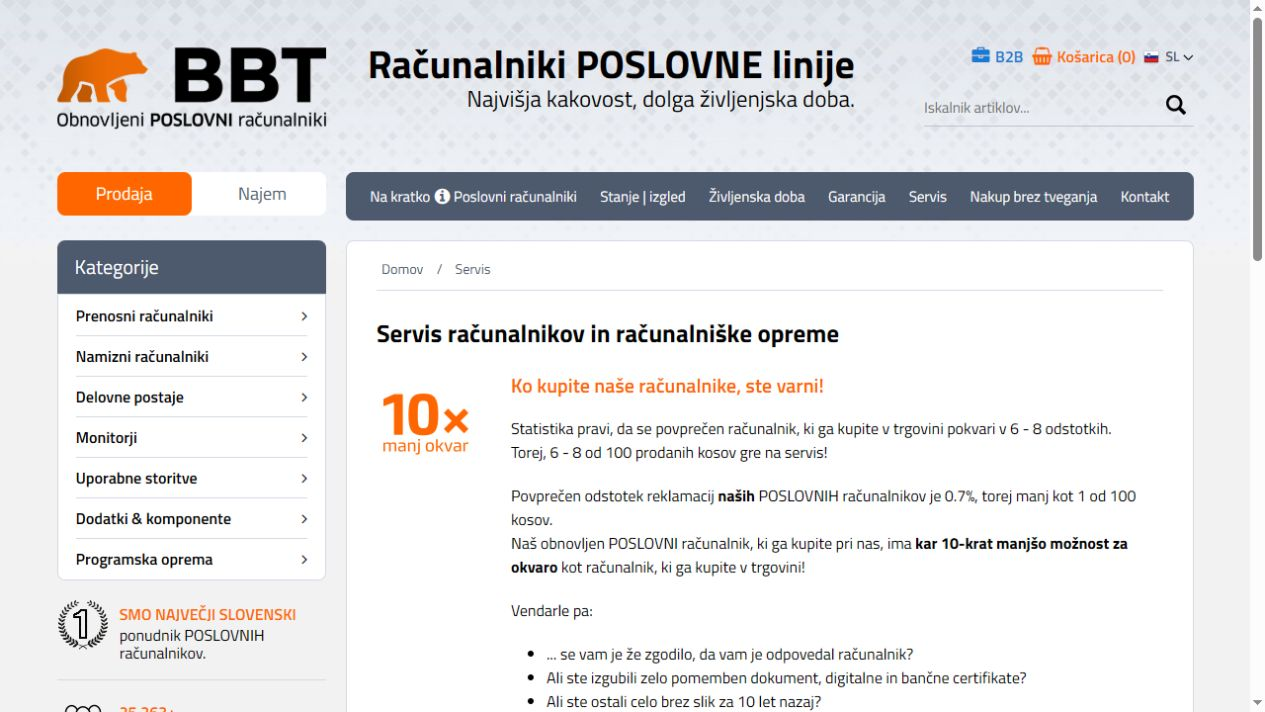
\includegraphics[width=\linewidth,height=83mm,keepaspectratio]{primer_bbt.png}
\caption{Predstavitev računalniškega servisa BBT. Lastni posnetek zaslona, 19.~11.~2026 \cite{bbt}.}
\label{fig:bbt}
\end{figure}

\newpage
\section{Zaključek}
Pregled kaže tri uporabne poudarke: ANNI izpostavi dostop do pomoči, Mlacom podrobno predstavi servisne stroške, BBT pa pojasni potek ob okvari \cite{anni,mlacom,bbt}. Pri ByteFixu bomo te ideje povezali v manjšo, pregledno predstavitveno stran.

Od obstoječih rešitev bomo prevzeli kratke predstavitve storitev, vidne kontaktne podatke, cenik ter pojasnilo postopka. Svojo rešitev bomo prilagodili obiskovalcu, ki želi najprej preveriti storitev in ceno, nato pa stopiti v stik. Na vseh zaslonih bo enaka navigacija, povezave iz storitev in cenika pa bodo vodile na O nas in kontakt.

Razlika bo predvsem v osredotočenem obsegu: brez trgovinskih kategorij, uporabniških računov in spremljanja servisnih nalog. Na domači strani bodo povzetek ponudbe in glavni poziv za stik, na ceniku pa jasno navedeno, da so cene informativne. Načrtovana prilagoditev manjšim zaslonom in razumljive oznake obrazca bosta podprli uporabo na telefonu.

Cilj ni dokazati, da bo ByteFix že v prvi različici boljši od uveljavljenih ponudnikov. Cilj je uporabniku olajšati orientacijo in pripraviti izvedljiv projekt za našo skupino. Izboljšave bomo preverjali pri nadaljnji izdelavi strani.

\begin{thebibliography}{9}
\bibitem{anni} ANNI, \emph{Domov -- Servis računalnikov in opreme}.
\url{https://servis.anni.si/}. Dostop: 19.~11.~2026.
\bibitem{mlacom} Mlacom, \emph{Storitve -- računalniški servis Ljubljana}.
\url{https://www.mlacom.si/storitve}. Dostop: 19.~11.~2026.
\bibitem{bbt} BBT, \emph{Servis računalnikov in računalniške opreme}.
\url{https://www.bbt.si/servis}. Dostop: 19.~11.~2026.
\end{thebibliography}
\end{document}
